% Summary of the thesis in paper style (two columns), same text as summary.tex.
% Figures: ../images (thesis) and figures/ (made by Code/figure_summary/*.py).
% Build: cd summary && latexmk -pdf -interaction=nonstopmode summary_paper.tex
\documentclass[10pt,a4paper,twocolumn]{article}
\usepackage[T1]{fontenc}
\usepackage[utf8]{inputenc}
\usepackage{lmodern}
\usepackage[hmargin=1.6cm,top=1.5cm,bottom=1.7cm,columnsep=0.55cm]{geometry}
\usepackage{microtype}
\usepackage{graphicx}
\usepackage{booktabs}
\usepackage{amsmath}
\usepackage[font=small,labelfont=bf]{caption}
\usepackage{balance}
\usepackage[hidelinks]{hyperref}
\graphicspath{{figures/}{../images/}}
\captionsetup{skip=4pt}
\setlength{\parskip}{0pt}
\setlength{\textfloatsep}{8pt plus 2pt minus 2pt}
\setlength{\dbltextfloatsep}{8pt plus 2pt minus 2pt}
\setlength{\intextsep}{6pt plus 2pt minus 2pt}
\setlength{\floatsep}{8pt plus 2pt minus 2pt}
\setlength{\dblfloatsep}{8pt plus 2pt minus 2pt}
\setcounter{dbltopnumber}{3}
\renewcommand{\topfraction}{0.9}
\renewcommand{\dbltopfraction}{0.9}
\renewcommand{\textfraction}{0.08}
\pagestyle{plain}
\emergencystretch=1.5em

\makeatletter
\renewcommand\section{\@startsection{section}{1}{\z@}{-1.4ex plus -0.5ex minus -0.2ex}{0.6ex plus 0.2ex}{\normalfont\large\bfseries}}
\makeatother

\begin{document}

\twocolumn[{%
\begin{center}
{\large\bfseries Vision-Based Row Following Navigation for Horticultural Robots\\with Automatically Labeled Semantic Segmentation\par}
\vspace{0.4em}
{Emanuele Pruiti (ID 347065)\par}
{\small Supervisors: Marcello Chiaberge, Alessandro Navone, Umberto Albertin\par}
\vspace{0.5em}
\begin{minipage}{0.84\textwidth}\small\noindent\textbf{Abstract.} A monocular RGB camera guides a robot between crop rows. The segmentation network is trained only on labels generated automatically by SAM~3, without manual correction. It guided the robot along a tomato row not present in its training data, with each of the five centerline extractors.\end{minipage}
\end{center}
\vspace{0.2em}
}]

\section{Introduction}

The demand for food is rising, while the shortage of skilled labor and the rising cost of farm management push agriculture towards autonomous robots. Row crops are among their most studied applications. A robot between two crop rows must stay in the corridor without damaging the plants, but dense canopies obstruct the GNSS signal and cause multi-path reflections. Greenhouse structures also obstruct it, and GNSS with RTK corrections and 3D LiDAR are costly. A monocular RGB camera is a cost-effective alternative. Classical camera pipelines isolate the plants with color indices and thresholds, which break with changes of light, shadows and weeds. Segmentation networks handle these conditions better, but they need many images annotated by hand at pixel level and must run fast on the onboard computer.

The work has three phases:
\begin{enumerate}\setlength{\itemsep}{0pt}
\item \textbf{Segmentation (Section~\ref{sec:segmentation}).} Choose a segmentation network that balances accuracy and speed on the robot and evaluate whether labels generated automatically by SAM~3, without manual correction, can replace manual annotation. The robot network is trained only on them.
\item \textbf{Extraction of the centerline (Section~\ref{sec:extraction}).} Develop two centerline extractors, Strip-IRLS and EdgeNet, and compare them with three baselines.
\item \textbf{Tests on the robot (Section~\ref{sec:robot}).} Run the complete chain on the robot Demetra and verify in a crop row, with all five extractors, that the network trained only on automatic labels can guide it.
\end{enumerate}

Figure~\ref{fig:pipeline} shows the complete chain that runs on the robot. For each camera frame, the chosen network predicts a mask of the path, the corridor between the rows. A centerline extractor turns this mask into a straight centerline, and a proportional controller steers the robot to keep the centerline at the center of the image. Segmenting first is also the idea behind EdgeNet, because a network that found the centerline directly in the camera images would need these images labeled with their centerline. EdgeNet instead finds it in the mask and is trained on generated masks whose centerline is known exactly, so with it no stage of the chain needs manual annotation, and it has no geometric parameters to tune.

\begin{figure*}[t]
  \centering
  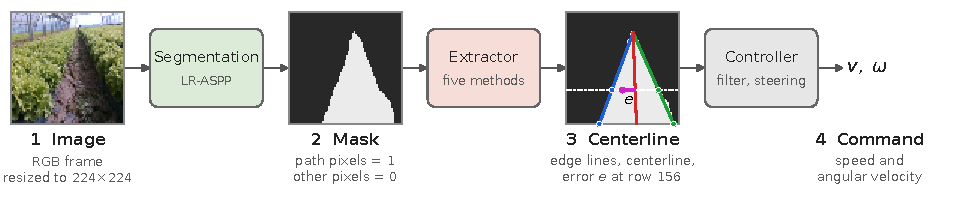
\includegraphics[width=0.75\linewidth]{pipeline_summary.pdf}
  \caption{Chain that runs on the robot for each camera frame. The network predicts the path mask, the extractor finds the centerline in it, and the controller computes the commands from the lateral error $e$.}
  \label{fig:pipeline}
\end{figure*}

\section{Segmentation trained on automatic labels}\label{sec:segmentation}

The images were recorded in a commercial greenhouse with the camera of the robot: 762 of lettuce, 878 of tomato and 319 of cucumber. Manual masks were drawn only for the lettuce images, because annotation is time-consuming and they were needed only as ground truth and to choose the network.

FCN, DeepLabV3 and LR-ASPP were fine-tuned from pretrained TorchVision weights on the manual lettuce masks, with four classes. FCN and DeepLabV3 reach an mIoU of 0.9253, 1.08 percentage points above LR-ASPP, while LR-ASPP is 7.2 times faster than FCN and 10.6 times faster than DeepLabV3 on the training GPU. With a similar accuracy, speed decided, because the network runs on the robot in real time, and LR-ASPP was chosen.

The automatic labels were generated offline by SAM~3, with one text prompt per class, and were used for training without inspection or correction. Three networks were trained on automatic lettuce labels, with four, three and two classes, and compared with the network trained on manual masks, on the same 77 lettuce test images. On all 77 images, their path IoU is only 0.39 to 0.41, because some images were taken from points outside the rows. There the automatic-label networks also mark soil that is not the path to follow, while the manual mask marks only that path, or nothing when there is none (Figure~\ref{fig:segmentation}a, bottom row). On the 42 test images taken between parallel rows, from viewpoints the robot can reach, in all three configurations the path IoU is 0.897 to 0.901, slightly lower than the 0.959 of the network trained on manual labels. The quality of the automatic labels depends on the class. Unlike the path, the covering material is segmented poorly (IoU of 0.17 against 0.83 on all 77 images), so they do not replace manual labels for every class, but they are enough for this work. The three configurations are almost equal and the extractors use only the path, so the robot uses a binary network.

After this result, the robot network, a binary LR-ASPP, was trained only on the automatic labels of all 1959 images of the three crops. A copy trained without the 77 lettuce test images reaches a path IoU of 0.907 between parallel rows. Figure~\ref{fig:segmentation}b shows the output of the robot network on tomato and cucumber.

\begin{figure*}[t]
  \centering
  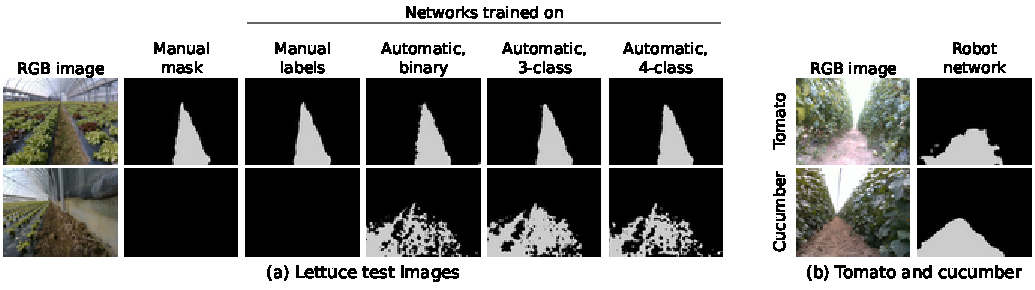
\includegraphics[width=0.85\linewidth]{segmentation_summary.pdf}
  \caption{Path masks. (a)~Lettuce test images with the manual mask and the output of the LR-ASPP networks trained on manual labels and on automatic labels with two, three and four classes. The bottom image is taken outside the rows, where the manual mask is empty and the automatic-label networks mark the soil as path. (b)~Output of the robot network on tomato and cucumber images, which have no manual mask.}
  \label{fig:segmentation}
\end{figure*}

\begin{table*}[t]
  \centering
  \footnotesize
  \caption{Offline results and time of the five extractors. Gross errors and \texttt{lost} masks are in \% of the masks of each group, which all contain a corridor.}
  \label{tab:summary}
  \setlength{\tabcolsep}{4pt}
  \begin{tabular}{@{}lccccc@{}}
    \toprule
     & \shortstack{Strip-IRLS\\(ours)} & \shortstack{EdgeNet\\(ours)} & \shortstack{RANSAC\\edges} & \shortstack{Center\\points} & \shortstack{Column\\histogram} \\
    \midrule
    \multicolumn{6}{@{}l}{\textit{Synthetic masks, one corridor (1900)}} \\
    Gross errors (\%) ($\downarrow$) & 0.3 & 0.1 & 0.1 & 1.0 & 23.0 \\
    \texttt{lost} (\%) ($\downarrow$) & 0.4 & 0.0 & 0.0 & 0.6 & 1.1 \\
    \midrule
    \multicolumn{6}{@{}l}{\textit{Synthetic masks, adjacent corridors (300)}} \\
    Gross errors (\%) ($\downarrow$) & 3.0 & 0.0 & 24.7 & 1.3 & 23.7 \\
    \texttt{lost} (\%) ($\downarrow$) & 1.3 & 8.3 & 0.0 & 0.0 & 0.3 \\
    \midrule
    \multicolumn{6}{@{}l}{\textit{Real frames with hand-marked edges (255)}} \\
    Gross errors (\%) ($\downarrow$) & 2.4 & 4.7 & 1.6 & 2.0 & 14.9 \\
    \texttt{lost} (\%) ($\downarrow$) & 2.0 & 0.8 & 2.0 & 3.1 & 5.5 \\
    \midrule
    \multicolumn{6}{@{}l}{\textit{Robot}} \\
    Time on the Jetson AGX Orin (ms) ($\downarrow$) & 11.07 & 4.68 & 15.52 & 7.27 & 0.91 \\
    \bottomrule
  \end{tabular}
\end{table*}

\section{Extraction of the centerline}\label{sec:extraction}

In this phase we developed two extractors, Strip-IRLS and EdgeNet, and compared them with three baselines. All five take the same $224\times224$ path mask and return a straight centerline, a confidence and a status (\texttt{ok}, \texttt{degraded} or \texttt{lost}). With \texttt{lost} the extractor returns no centerline, and if this lasts more than 0.5~s the robot stops.

\textbf{Strip-IRLS (ours)} divides the lower part of the mask into horizontal strips. Going up from the bottom, it links in each strip the path interval that continues the corridor found below and keeps the chain with the most edge samples. It fits the two edges with iteratively reweighted least squares, and the centerline is their mean.

\textbf{EdgeNet (ours)} is a small network of about 0.8 million parameters that regresses the two corridor edges from the mask. It is trained only on generated masks with exact edges and with errors like those of the segmentation, such as holes and blobs, so it needs no manual annotation. Apart from the confidence thresholds that decide the status, it has no parameters to set by hand.

\textbf{Baselines:} Center points (one line fitted through the midpoints of the path in horizontal strips of the mask), Column histogram (the column with the most path pixels) and RANSAC edges (the two edges fitted with RANSAC on the row extremes of the corridor).


The extractors were tested on 2400 synthetic masks with an exact centerline and on 255 real frames whose corridor edges were marked by hand. There is no clear winner, and finding one was not the aim. Synthetic masks were used both to tune the parameters, on a separate set, and to show how the extractors behave in the different scenarios and which scenarios cause them the most problems. For the masks with one corridor and for those with adjacent corridors, Table~\ref{tab:summary} gives the gross errors (centerline errors above 15~px at the row read by the controller) and the \texttt{lost} masks (the mask has a corridor but the extractor returns no centerline). On the masks with one corridor, Strip-IRLS, EdgeNet and RANSAC edges have the fewest gross errors (0.1 to 0.3\%). Adjacent corridors are the hardest synthetic case for RANSAC edges, with 24.7\% of gross errors against 3.0\% for Strip-IRLS and 1.3\% for Center points. EdgeNet has none, and its 8.3\% of \texttt{lost} masks come only from its confidence, which falls below the threshold of \texttt{lost} although its line is correct. On the 255 real frames, Strip-IRLS, EdgeNet and RANSAC edges also have few gross errors, 6, 12 and 4. These 22 errors fall on only 15 frames, so the three fail mostly on the same masks, where the segmentation is much worse than on the others. Center points has few errors there too, 5 gross errors and 8 \texttt{lost} frames. Column histogram is the fastest, but has many gross errors in every group (14.9 to 23.7\%). On the Jetson, Strip-IRLS is 1.4 times and EdgeNet 3.3 times faster than RANSAC edges.

\begin{table*}[t]
  \centering
  \footnotesize
  \caption{Field tests: lateral distance of the robot from the row centerline (cm), from 12 to 4~m (short runs) and from 15 to 39~m (full row) from the station. RMSE: distance from the centerline. Std runs: difference between the runs of an extractor. RMSD: difference from the other four. Short runs: mean RMSE and largest Max of the three runs.}
  \label{tab:field}
  \setlength{\tabcolsep}{4pt}
  \begin{tabular}{@{}lccccccc@{}}
    \toprule
     & \multicolumn{4}{c}{Short runs (3 per extractor)} & \multicolumn{3}{c}{Full row (1 per extractor)} \\
    \cmidrule(lr){2-5}\cmidrule(lr){6-8}
    Extractor & RMSE ($\downarrow$) & Max ($\downarrow$) & Std runs ($\downarrow$) & RMSD & RMSE ($\downarrow$) & Max ($\downarrow$) & RMSD \\
    \midrule
    Strip-IRLS (ours) & 5.7 & 11.0 & 0.6 & 1.5 & 9.1 & 20.4 & 1.9 \\
    EdgeNet (ours) & 5.3 & 10.5 & 0.3 & 1.1 & 8.4 & 16.3 & 1.9 \\
    RANSAC edges & 5.4 & 10.1 & 0.6 & 1.8 & 9.4 & 18.4 & 1.6 \\
    Center points & 5.7 & 10.8 & 0.4 & 1.6 & 9.2 & 17.5 & 1.9 \\
    Column histogram & 5.5 & 13.6 & 4.3 & 5.1 & 8.5 & 17.4 & 4.1 \\
    \bottomrule
  \end{tabular}
\end{table*}

\begin{figure*}[t]
  \centering
  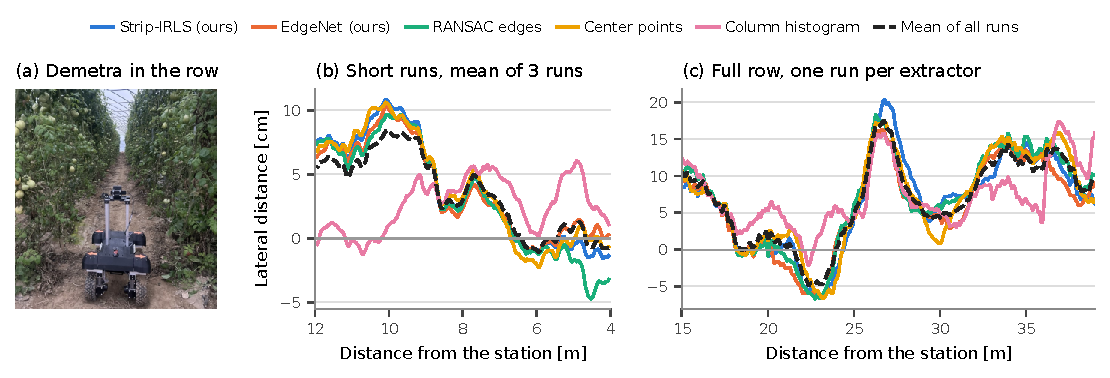
\includegraphics[width=0.9\linewidth]{field_summary_paper.pdf}
  \caption{(a)~Demetra in the tomato row. (b, c)~Lateral distance from the row centerline, with the robot moving from left to right. (b)~Mean of the three short runs of each extractor, at 0.20~m/s. (c)~Full row at 0.50~m/s, one run per extractor.}
  \label{fig:field}
\end{figure*}

\section{Tests on the robot}\label{sec:robot}

Demetra, the four-wheel-steering robot of the tests, has an NVIDIA Jetson AGX Orin. Without the debug video, a frame is processed in 11.3 to 26.2~ms depending on the extractor, less than the 33.3~ms frame period of the camera.

The field tests were made on 4 November 2026 in a greenhouse, in a tomato row not present in the training data of the robot network, with sparse plants and poor light (Figure~\ref{fig:field}a). The trajectory of the robot was measured with a total station. Each extractor made three short runs at 0.20~m/s, starting from a position set by hand and compared between 12 and 4~m from the station (Figure~\ref{fig:field}b), and one run along the full row at 0.50~m/s, compared from 15 to 39~m (Figure~\ref{fig:field}c). Between runs only the extractor changed. The row centerline passes through five points placed by eye on the center of the row, so it is not accurate to the centimeter.

The RMSE shows how close the robot stays to the row centerline, the standard deviation between runs how repeatable each extractor is, and the RMSD how similar its mean trajectory is to that of the other four extractors. The last two are differences between runs at the same positions, so the error of the row centerline cancels in them.

With all five extractors the robot followed the center of the row without touching the plants (Figure~\ref{fig:field} and Table~\ref{tab:field}). Its RMSE from the row centerline is about 5.5~cm on the short runs and 9~cm on the full row, and its largest distance 20.4~cm, in a row about 1~m wide. Strip-IRLS, EdgeNet, RANSAC edges and Center points drove the robot along almost the same trajectory. Their mean trajectories differ by less than 2~cm (RMSD), and each of them repeats its own runs within 0.6~cm (standard deviation between runs). Their distance from the centerline repeats at the same positions in all their runs, so it most likely comes from the row itself, where the plants reach into the path or the predicted path widens, and from the errors of the row centerline, not from the extractor. Column histogram is the exception. Its RMSE is close to that of the others, and along the full row it follows their trajectory, up to 10~cm away, but its three short runs follow different curves (standard deviation between runs of 4.3~cm). Where the predicted path covers most of the width of the mask, the column with the most path pixels can lie at the image border.

\balance
\section{Conclusions}

Automatic labels, used without correction, can replace manual annotation for the path between parallel rows, with a path IoU about 6 percentage points lower, but not for every class. A network trained only on these labels guided the robot along a tomato row not present in its training data, with each of the five extractors. With EdgeNet, no stage of the chain needs manual annotation, and the extraction has no geometric parameters to set by hand. The segmentation network learns from automatic labels, EdgeNet from generated masks, and EdgeNet performs like the best geometric extractors. Strip-IRLS and EdgeNet have few gross errors, like RANSAC edges, and run faster on the Jetson, and with adjacent corridors they also have fewer gross errors. Strip-IRLS, EdgeNet and RANSAC edges fail mostly on the same badly segmented frames, and in the field four extractors drove the robot along almost the same trajectory, so the quality of the segmentation affects the result more than the choice among these extractors.

The segmentation was measured against manual masks only on lettuce, with a random split by image, so the results can be optimistic. The robot network was trained on all the images, so an independent measure needs manual masks of new images. The confidence of the extractors does not always follow the error, so some gross errors do not warn the controller. The chain also has no explicit detection of obstacles on the path. The field tests cover one row of one crop on one day. A next step is to let the robot navigate the whole greenhouse, whatever the layout of its rows, and not only along one row.

\end{document}
